% applications/bimalignment-DE.tex
\chapter{BIM-Alignment-Modellierung}
\label{chap:applications-bimalignment}

Dieses Kapitel ordnet BIMalignment als Interoperabilitäts- und
Arbeitsablaufanwendung von AIM ein, nicht als konkurrierende kanonische
Architektur.

\section{Anwendungskontext}

BIM- und Austauschstandards (beispielsweise IFC, LandXML und GIS-gekoppelte
Container) sind wesentliche Mechanismen der Projektinteroperabilität. In
AIM werden sie als Repräsentations- und Austauschebenen behandelt, die der
kanonischen Ingenieursemantik nachgelagert sind.

Die erste Abbildung beantwortet die Grenzfrage dieses Kapitels: Welche
semantische Ebene besitzt die Ingenieurbedeutung, und welche stellt diese
Bedeutung lediglich für den Austausch dar?

\begin{figure}[ht]
\centering
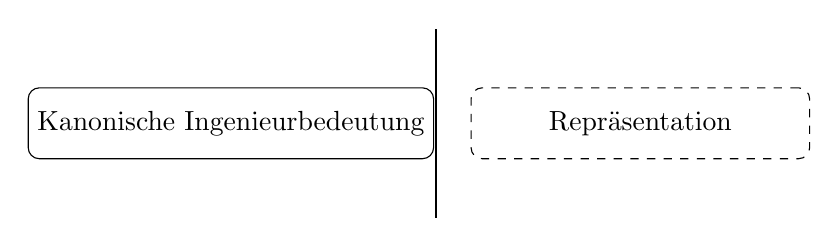
\begin{tikzpicture}[
  box/.style={draw, rounded corners, minimum width=4.3cm, minimum height=0.9cm, align=center},
  sec/.style={draw, rounded corners, dashed, minimum width=4.3cm, minimum height=0.9cm, align=center}
]
  \node[box] (canon) at (-2.6,0) {Kanonische Ingenieurbedeutung};
  \node[sec] (repr) at (2.6,0) {Repräsentation};
  \draw[thick] (0,-1.2) -- (0,1.2);
\end{tikzpicture}

\caption{Unterstützender Vergleich: Kanonische Ingenieurbedeutung und Repräsentation sind verschiedene Ebenen.}
\label{fig:support-canonical-vs-representation}
\end{figure}

Die ingenieurwissenschaftliche Konsequenz ist, dass BIM-Arbeitsabläufe
kanonischen AIM-Zustand und kanonische Operatoren verwenden müssen, statt
sie in Austauschschemata neu zu definieren.

\section{Rolle der AIM-zu-BIM-Integration}

BIMalignment bezeichnet in dieser Arbeit eine Alignment-zentrierte
Integration, bei der AIM kanonische Semantik sowie Laufzeit- und
Realisierungsauswertung bereitstellt, während BIM-orientierte Strukturen
objektorientierte Repräsentation, Arbeitsablaufintegration und Austausch
über den Lebenszyklus ermöglichen.

\begin{principle}[BIM-Integrationsprinzip]
Die BIM-Integration verwendet kanonische AIM-Begriffe und belässt deren
Zuständigkeit außerhalb der Anwendungskapitel.
\end{principle}

\section{Interpretation der Verarbeitungskette}

Eine typische Interpretationskette lautet
\[
\text{Austausch/Import}
\rightarrow
\substack{\text{AIM-Normalisierung}\\\text{und -Auswertung}}
\rightarrow
\text{Anwendungsfolge}
\rightarrow
\text{Repräsentation/Export}.
\]

Damit bleiben Ingenieurobjekte und Repräsentationen begrifflich getrennt.

Die nächste Abbildung behandelt die Interoperabilitätsfrage: Wie lassen
sich native und importierte Alignments unter einer gemeinsamen
kanonischen Zustandssemantik konsistent interpretieren?

\begin{figure}[ht]
\centering
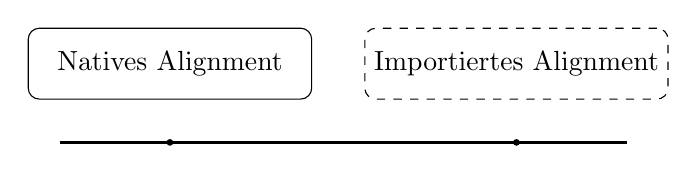
\begin{tikzpicture}[
  box/.style={draw, rounded corners, minimum width=3.6cm, minimum height=0.9cm, align=center},
  imp/.style={draw, rounded corners, dashed, minimum width=3.6cm, minimum height=0.9cm, align=center}
]
  \node[box] (native) at (-2.2,0) {Natives Alignment};
  \node[imp] (imported) at (2.2,0) {Importiertes Alignment};
  \draw[thick] (-3.6,-1.0) -- (3.6,-1.0);
  \filldraw (-2.2,-1.0) circle (1.0pt);
  \filldraw (2.2,-1.0) circle (1.0pt);
\end{tikzpicture}

\caption{Unterstützender Vergleich: Native und importierte Alignments erfordern eine gemeinsame kanonische Interpretation.}
\label{fig:support-native-vs-imported}
\end{figure}

Die Folge ist operativ: Importqualität wird anhand der Kompatibilität mit
der kanonischen Semantik bewertet, nicht allein anhand der Ähnlichkeit auf
Formatebene.

\section{Klärung der Grenze}

BIMalignment wird nicht als paralleles Zustandsmodell dargestellt. Es ist
eine anwendungsorientierte Integrationsstrategie, die von kanonischer
Alignment-Semantik, pose2/pose3-Interpretation, metrischer und physischer
Realisierung sowie Laufzeitdiensten abhängt.

\section{Verbindung zu AIM}
\begin{summary}
BIMalignment ist in dieser Arbeit eine nachgelagerte
Interoperabilitätsanwendung von AIM.

Sie zeigt, wie kanonische, Alignment-zentrierte Ingenieursemantik mit
BIM/GIS-Austauschökosystemen verbunden werden kann, ohne die begriffliche
Zuständigkeit von der genehmigten Kernel-Architektur zu verlagern.
\end{summary}
